\section{One same-information reconstruction control}
\label{sec:comparison}
The preceding replacement fixes learning error but retains the aggregator.
We now test whether a different interpretation can exploit information already
present in neighboring coarse values. Development uses the consumed 2,000-scene
IID discovery bank. One implementation and two scalar offsets are fixed before
evaluating the already consumed 2,000-scene confirmation bank. This is an
\emph{appended baseline analysis}, not a new untouched confirmation. There is
no new training, dataset, resolution search, or risk certification.

\paragraph{Three treatments with identical action access.}
The primary track uses the perfect actual target 64 field; the secondary track
uses all five existing restored model fields. Uniform interpretation computes
the original exposure. All three treatments may access exactly the same F512,
so PLIC is not given better action geometry. The global shift subtracts one
constant after Eq.~\ref{eq:cost}. Its argmin is the original uniform argmin,
since translation preserves ranking; no clipping-induced ties are introduced.
From a fixed 13-value offset bank, development maximizes safe-accepted count
subject to no increase in observed unsafe-accepted count relative to uniform.
Ties favor the smallest absolute offset. The selected offset is .001 for the
target track and zero shared across the five learned models.

The only spatial alternative is the established Parker--Youngs PLIC construction
\citep{pilliod2004}. A fixed weighted 3$\times $3 gradient with center weight 2
estimates a cell's outward normal. A straight half-plane then matches the cell's
original fraction by analytic square-area inversion. Empty/full cells remain
unchanged; cells with gradient L1 norm at most $10^{-12}$ retain uniform occupancy
rather than an invented orientation. Exact line-cut fractions of fine pixel
squares are integrated against F512. Coarse predictions are neither thresholded
nor denoised. The reconstruction routine accepts only the coarse field and
footprints, never true patch parameters, fine property masks, reference costs,
or oracle boundary normals. It is a first-order PLIC baseline, not the
second-order ELVIRA method or a newly proposed algorithm.

\paragraph{Full-scene gains and harms.}
Table~\ref{tab:appended} reports every scene, including no-safe-candidate cases,
and both recovered and newly harmed decisions. PLIC recovers 44 of the target
oracle's 54 lost opportunities without newly losing a previously accepted safe
one. However, it introduces 16 unsafe accepts: total unsafe count rises from 2
to 18. Safe opportunity efficiency rises from 96.61\% to 99.37\%, while empirical
unsafe frequency among accepted rises from .13\% to 1.13\%. The frozen shift
recovers six opportunities and introduces three unsafe accepts.

\begin{table}[t]
\centering\small
\caption{Appended full-scene comparison relative to uniform interpretation.
Target counts use 2,000 scenes. Learned counts aggregate five models sharing
those scenes and are not 10,000 independent trials. ``New unsafe'' counts newly
unsafe accepted decisions; no previously unsafe accepts are resolved on this bank.}
\label{tab:appended}
\begin{tabular}{llrrrrr}
\toprule
Input & Interpretation & Recovered & New safe loss & New unsafe & $R$ & $\eta $\\
\midrule
Target 64 & Uniform &0&0&0&.13\%&96.61\%\\
 & Global shift &6&0&3&.32\%&96.98\%\\
 & PLIC &44&0&16&1.13\%&99.37\%\\
\midrule
Five models & Uniform &0&0&0&1.03\%&96.77\%\\
 & Global shift &0&0&0&1.03\%&96.77\%\\
 & PLIC &83&0&43&1.56\%&97.81\%\\
\bottomrule
\end{tabular}
\end{table}

The learned track also has a mixed outcome. PLIC recovers 83 safe model--scene
decisions and adds 43 unsafe accepts, with no new safe loss observed. Net safe
acceptance increases .83 pp (descriptive crossed 95\% interval [.51,1.19] pp), while
new unsafe acceptance increases .43 pp ([.20,.69] pp). The target track's net safe
gain is 2.20 pp ([1.60,2.85] pp). The selected learned shift is zero and changes no
outcome. Fixed-selection analysis yields the same recovery and new-unsafe totals
on this appended bank, so those totals are not explained solely by permission
to reselect; the event archive retains action identities and individual changes.

\begin{figure}[t]
\centering
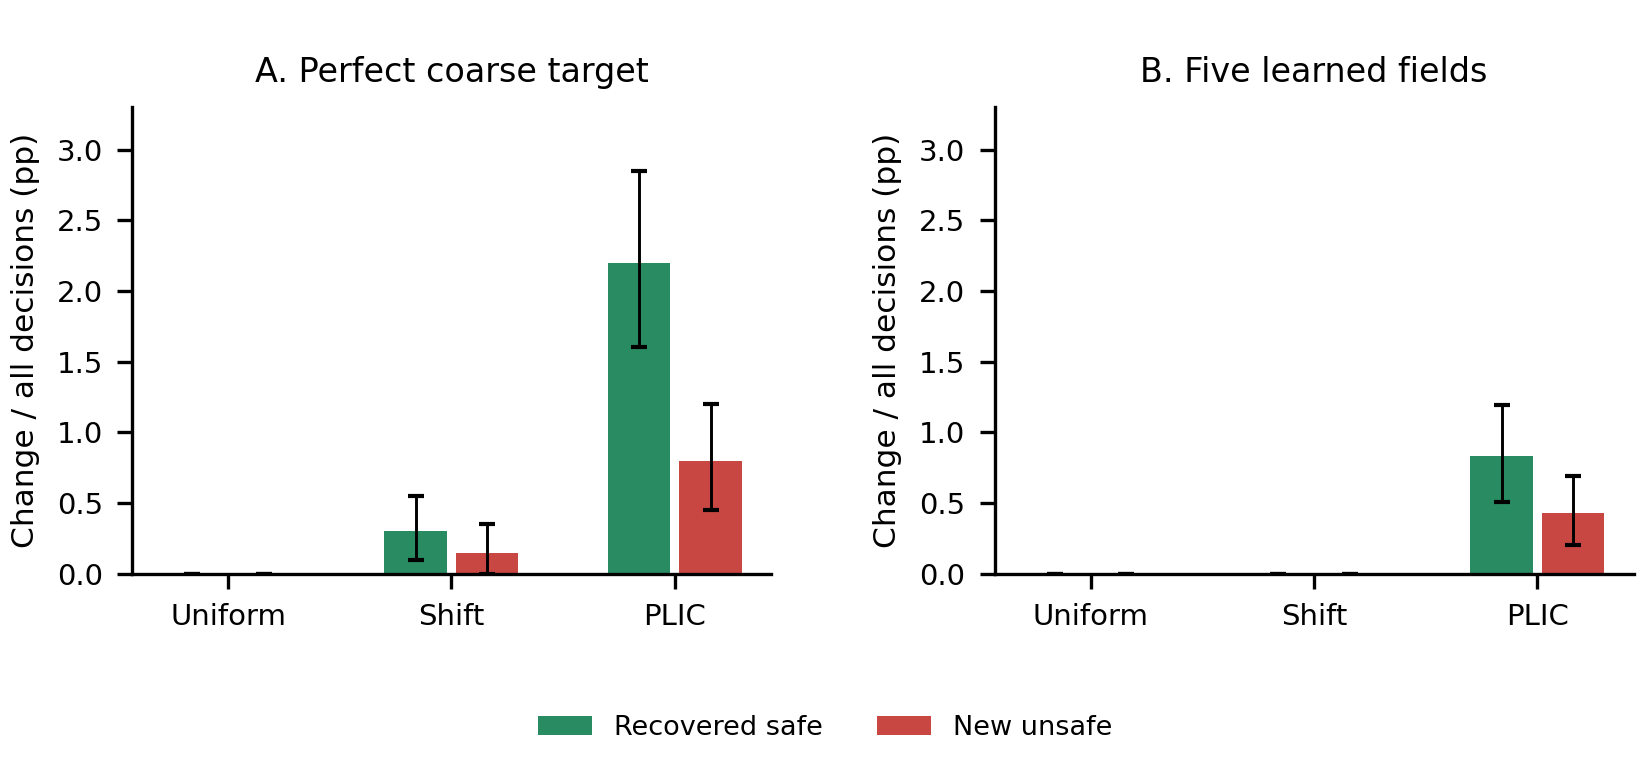
\includegraphics[width=\linewidth]{figures/same_information_tradeoff.png}
\caption{Opportunity recovery and newly unsafe acceptance must be read together.
PLIC uses the same coarse field and action information as uniform integration.
No new safe losses were observed, but both input tracks add unsafe accepts.
The offset was fitted under a development unsafe-count constraint that was not
imposed on PLIC; these selected points are not a matched-risk comparison.}
\label{fig:appended}
\end{figure}

\paragraph{A concrete cancellation failure.}
For 25 of the 43 newly unsafe learned decisions, the action stays unchanged,
baseline model and target-measurement errors have opposite signs, target-measurement
absolute error decreases under PLIC, and total absolute error increases. These
conditions are checked on each event, not inferred from aggregate means. For
the first such event in scene/model order, Table~\ref{tab:cancellation} shows
that both component absolute cost errors improve, yet their earlier
opposition disappears and the total underestimation worsens. All 43 events,
including the 18 not meeting this joint pattern, are retained. The example
supports a particular failure mechanism, not a claim that cancellation explains
every harmful change.

\begin{table}[t]
\centering\small
\caption{First event satisfying the stated cancellation pattern, in scene/model order. The same reference-unsafe action is rejected before reconstruction and accepted after it ($\tau=.02$). This is a conditional illustration; all 43 newly unsafe learned events remain in the archive.}
\label{tab:cancellation}
\begin{tabular}{lrr}
\toprule
Quantity on the same action & Uniform & PLIC\\
\midrule
Reference cost & +0.024972 & +0.024972\\
Target estimate & +0.031961 & +0.021431\\
Learned estimate & +0.021279 & +0.016964\\
Target-measurement cost error & +0.006989 & -0.003541\\
Model-relative-to-target cost error & -0.010682 & -0.004467\\
Total cost error & -0.003693 & -0.008008\\
Decision & Reject & Accept (unsafe)\\
\bottomrule
\end{tabular}
\end{table}


\paragraph{What this comparison establishes.}
The recovery demonstrates that the current coarse field contains spatial
structure usable by another interpretation; the original residual loss cannot
simply be called irreducible representation error. It does not demonstrate a
risk-free repair or universal superiority over scalar calibration. The chosen
offset is constrained not to add development unsafe outcomes, whereas PLIC is
not. The full development shift curve is therefore disclosed in
Appendix~\ref{app:shift}: larger offsets recover more opportunities at higher
risk. We do not tune another offset on the appended bank. The conclusion is to
separate supervision fidelity, spatial interpretation, and acceptance calibration,
and to re-evaluate the latter after changing the former. No earlier certificate
is inherited by either modified rule.
